%!TEX root = oral.tex

\section{Role of dynamic pricing in Uber}

	\begin{frame}
	\textbf{Paper 3: Surge Pricing Solves the Wild Goose Chase}
	\begin{itemize}
		\item Juan Camilo Castillo \\
		\textit{Stanford University}
		\item Dan Knoepfle \\
		\textit{Uber Technologies}
		\item E. Glen Weyl \\
		\textit{Microsoft Research}
	\end{itemize}
	\end{frame}

    \begin{frame}{Ride Hailing}
    \begin{itemize}
        \item Uber, Lyft: more efficient matching technology than taxis
        \begin{itemize}
            \item \textcite{cramer2016disruptive}: Utilization rate increases by 30--50\%
            \item Potential welfare gain is substantial \\
        \end{itemize}
        \pause
        \item Challenges to get market design right
        \begin{itemize}
            \item Matching passengers with drivers
            \item Pricing (dynamic?)
        \end{itemize}
    \end{itemize}
    % \pause
    % \alert{Surge Pricing solves a matching failure!}
    \end{frame}

    \begin{frame}{Wild Goose Chases (WGCs)}
    Ride-hailing systems are prone to \textit{wild goose chases}
    \pause
    \begin{itemize}
        \item Too many ride requests
        \item Drivers spend more time picking up passengers
        \item Number of completed trips drop
    \end{itemize}
    \pause
    \metroset{block=fill}
    \only<3>{
    \begin{block}{Driver Life:}
    	\centering
    	\large{Idle Time} $\rightarrow$ \large{Pickup Time} $\rightarrow$ \large{Travel Time}
    \end{block}
    }
    \pause
    \only<4->{
    \begin{block}{Driver Life:}
    	\centering
    	\large{Idle Time} $\rightarrow$ \alert{\large{Pickup Time}} $\rightarrow$ \large{Travel Time}
    \end{block}
    }
    % \pause
    % \only<3>{\alert{Street-hail cabs do not face the same problem!}}
    \pause
    Research problem: How to avoid Wild Goose Chases?
    \pause
    \begin{itemize}
        \item WGCs can be avoided by setting higher prices
        %\item With uniform pricing: higher costs \textit{always}
        %\item With dynamic pricing: lower costs during low demand
    \end{itemize}
    \end{frame}

    \begin{frame}{Notations}
    	\begin{itemize}
    		\item $T$ : Waiting time for customer = Pickup time for driver
    		\pause
    		\item $p$ : Price point
    		\pause
    		\item $L$ : Labor supply (total number of drivers)
    		\pause
    		\item $Q$ : Quantity (total number of completed rides)
    		\pause
    		\item $D(T, p)$ : Demand function
    		\pause
    		\item $S(T, L)$ : Supply function
    	\end{itemize}
    \end{frame}

    \begin{frame}{Demand}
        \begin{figure}
            \centering
            {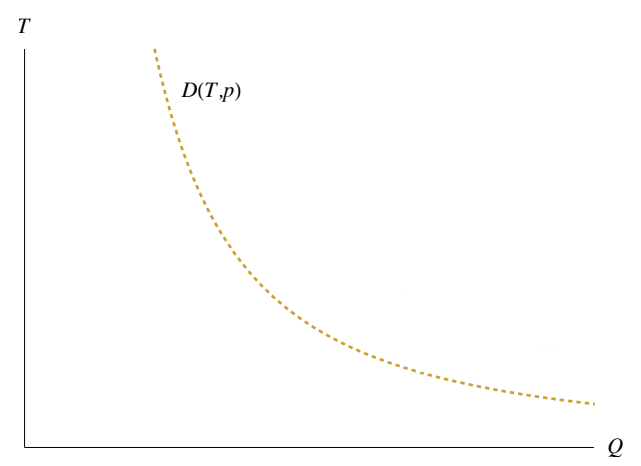
\includegraphics[scale=0.30]{plots/demand.png}}
            \caption{Demand curve\footcite{castillo2017surge}.}
        \end{figure}
    \end{frame}

    \begin{frame}{Supply}
        \begin{figure}
            \centering
            {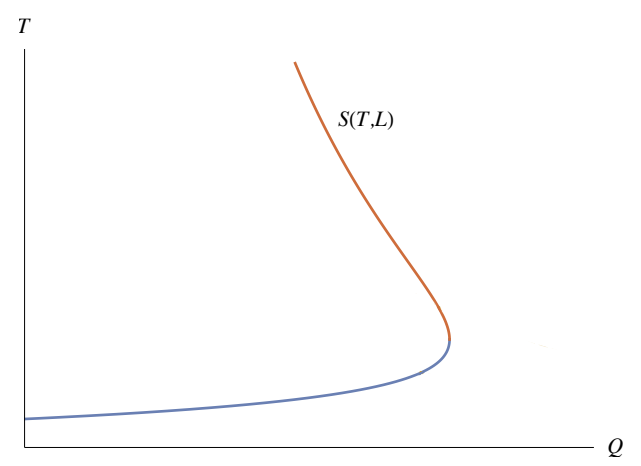
\includegraphics[scale=0.30]{plots/supply.png}}
            \caption{Supply curve\footcite{castillo2017surge}.}
        \end{figure}
    \end{frame}

    \begin{frame}{Empirical supply}
        \begin{figure}
            \centering
            {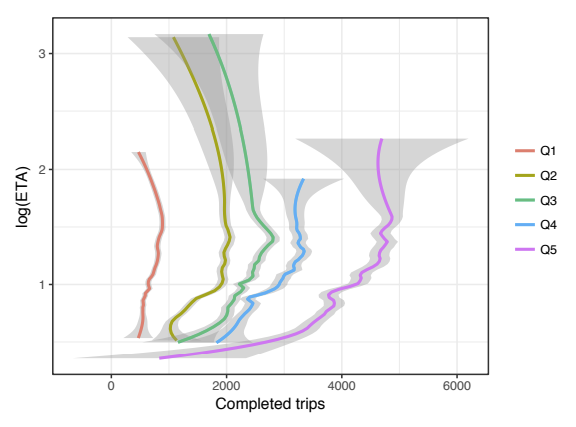
\includegraphics[scale=0.35]{plots/empirical_supply.png}}
            \caption{Quintiles of empirical supply\footcite{castillo2017surge}.}
        \end{figure}
    \end{frame}

    \begin{frame}{Equilibrium}
        \begin{figure}
            \centering
            {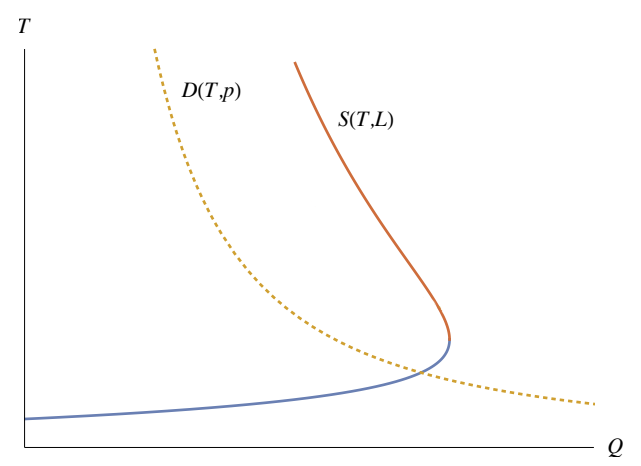
\includegraphics[scale=0.30]{plots/equilibrium.png}}
            \caption{Equilibrium point\footcite{castillo2017surge}.}
        \end{figure}
    \end{frame}

    \begin{frame}{Equilibrium}
        \begin{figure}
            \centering
            {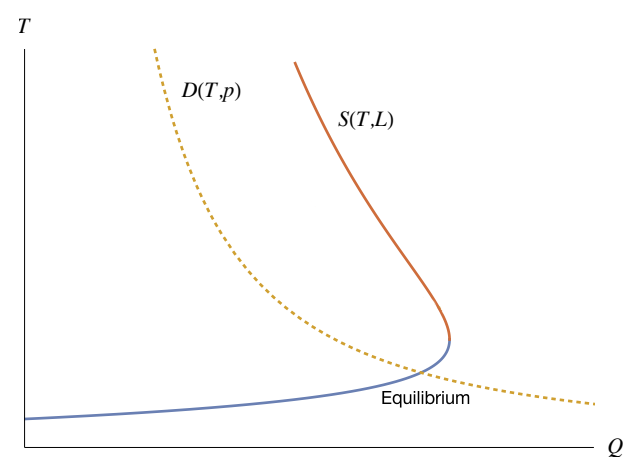
\includegraphics[scale=0.30]{plots/equilibrium_0.png}}
            \caption{Equilibrium point.}
        \end{figure}
    \end{frame}

    % \begin{frame}{Wild Goose Chase}
    %     \begin{figure}
    %         \centering
    %         {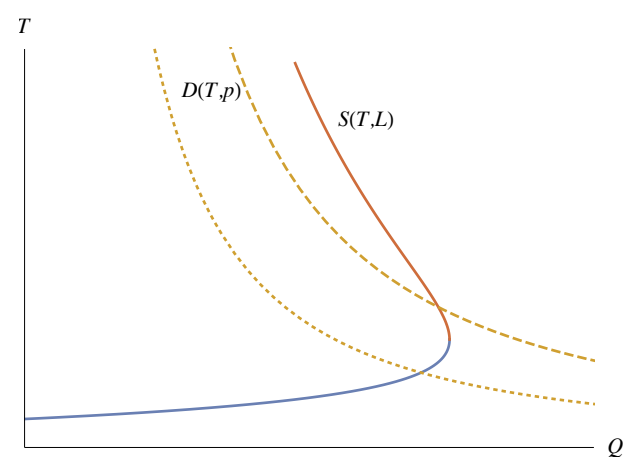
\includegraphics[scale=0.30]{plots/wild_goose_chase.png}}
    %         \caption{Wild Goose Chase\footcite{castillo2017surge}.}
    %     \end{figure}
    % \end{frame}

    \begin{frame}{Wild Goose Chase}
        \begin{figure}
            \centering
            {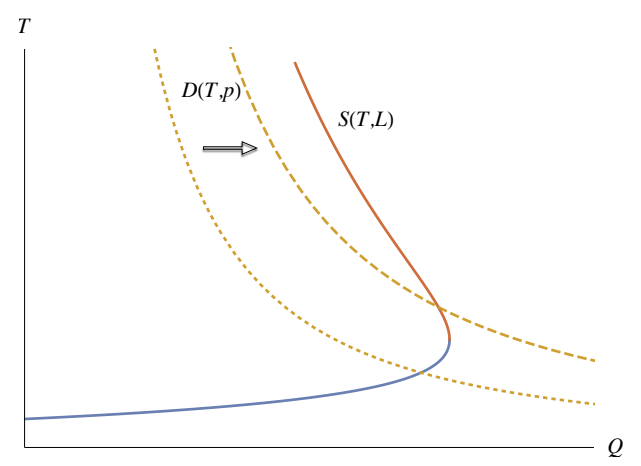
\includegraphics[scale=0.30]{plots/wild_goose_chase_0.png}}
            \caption{Wild Goose Chase.}
        \end{figure}
    \end{frame}

    \begin{frame}{Wild Goose Chase}
        \begin{figure}
            \centering
            {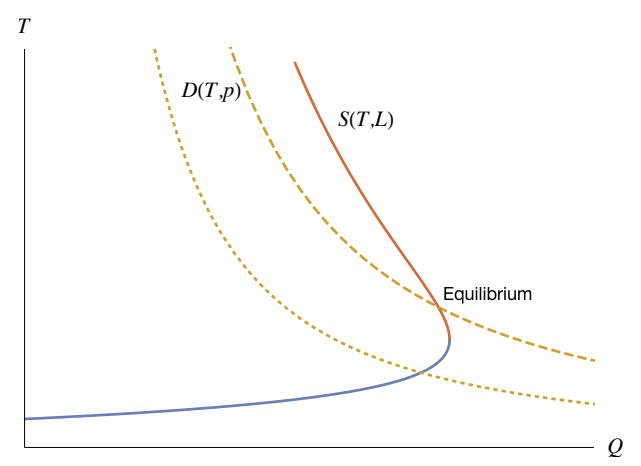
\includegraphics[scale=0.30]{plots/wild_goose_chase_1.png}}
            \caption{Wild Goose Chase.}
        \end{figure}
    \end{frame}

    % \begin{frame}{Market Collapse}
    %     \begin{figure}
    %         \centering
    %         {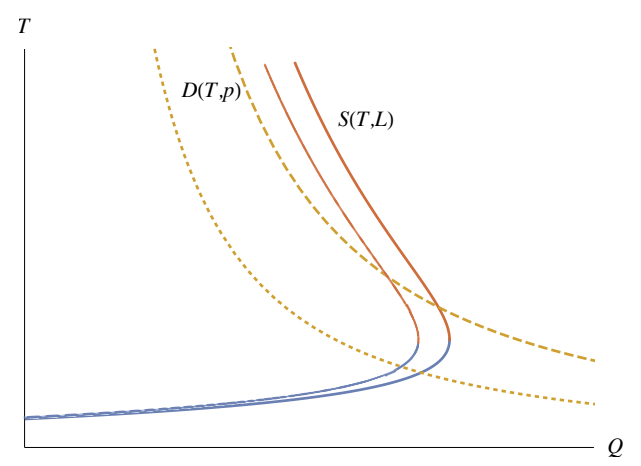
\includegraphics[scale=0.30]{plots/market_collapse.png}}
    %         \caption{Market Collapse\footcite{castillo2017surge}.}
    %     \end{figure}
    % \end{frame}

    \begin{frame}{Market Collapse}
        \begin{figure}
            \centering
            {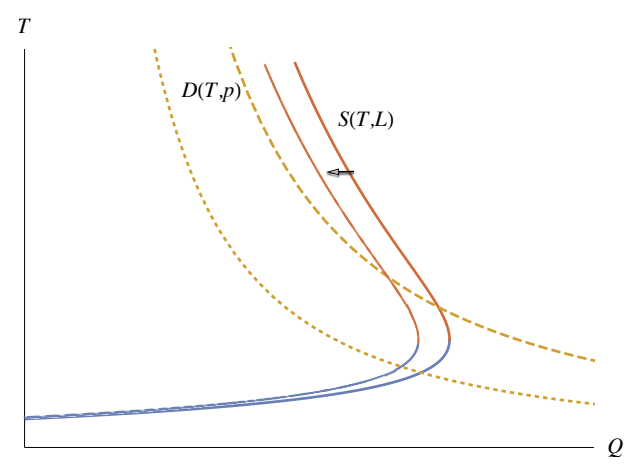
\includegraphics[scale=0.30]{plots/market_collapse_0.png}}
            \caption{Market Collapse.}
        \end{figure}
    \end{frame}

    \begin{frame}{Market Collapse}
        \begin{figure}
            \centering
            {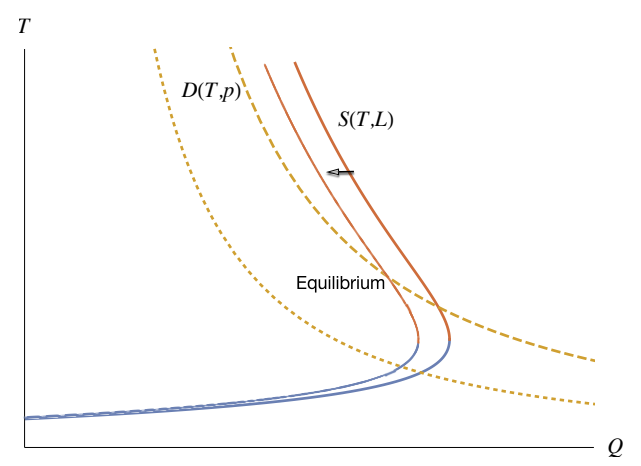
\includegraphics[scale=0.30]{plots/market_collapse_1.png}}
            \caption{Market Collapse.}
        \end{figure}
    \end{frame}

    \begin{frame}{Pricing for Strong vs. Weak Market}
    	\large{Welfare = Customer Utility + Driver earnings + Platform earnings} \\
    	\pause
    	\textbf{Weak market} = low demand (11am-noon) \\
    	\textbf{Strong market} = high demand (6pm-7pm)
    	\pause
    	\only<3>{
        \begin{figure}
            \centering
            {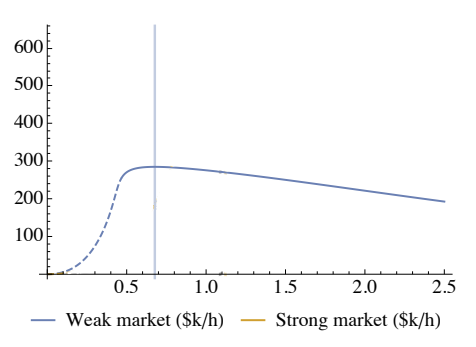
\includegraphics[scale=0.35]{plots/weak_strong_market_0.png}}
            \caption{Need for dynamic pricing\footcite{castillo2017surge}.}
        \end{figure}
        }
        \pause
        \only<4>{
        \begin{figure}
            \centering
            {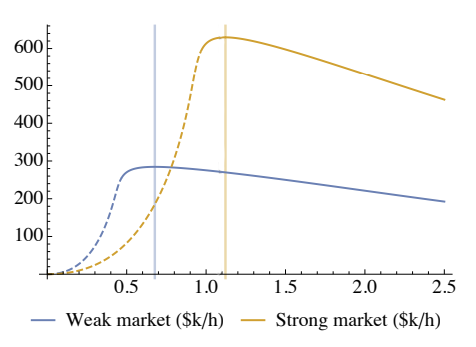
\includegraphics[scale=0.35]{plots/weak_strong_market_1.png}}
            \caption{Need for dynamic pricing\footcite{castillo2017surge}.}
        \end{figure}
        }
    \end{frame}

    \begin{frame}{Summary}
    	\textbf{Positives:}
    	\begin{itemize}
    		\item Formulation of endogenous relationship between supply and demand.
    	\end{itemize}
    		\vspace{0.1in}
    		\pause
    	\textbf{Concerns:}
    	\begin{itemize}
    		\item \alert{Location-based discrimination?}
    		\item \alert{Oblivious to re-balancing problem. Uber POV - surge pricing helps with re-balancing.}
    	\end{itemize}
    \end{frame}